\PassOptionsToPackage{unicode=true}{hyperref} % options for packages loaded elsewhere
\PassOptionsToPackage{hyphens}{url}
%
\documentclass[]{article}
\usepackage{lmodern}
\usepackage{amssymb,amsmath}
\usepackage{ifxetex,ifluatex}
\usepackage{fixltx2e} % provides \textsubscript
\ifnum 0\ifxetex 1\fi\ifluatex 1\fi=0 % if pdftex
  \usepackage[T1]{fontenc}
  \usepackage[utf8]{inputenc}
  \usepackage{textcomp} % provides euro and other symbols
\else % if luatex or xelatex
  \usepackage{unicode-math}
  \defaultfontfeatures{Ligatures=TeX,Scale=MatchLowercase}
\fi
% use upquote if available, for straight quotes in verbatim environments
\IfFileExists{upquote.sty}{\usepackage{upquote}}{}
% use microtype if available
\IfFileExists{microtype.sty}{%
\usepackage[]{microtype}
\UseMicrotypeSet[protrusion]{basicmath} % disable protrusion for tt fonts
}{}
\IfFileExists{parskip.sty}{%
\usepackage{parskip}
}{% else
\setlength{\parindent}{0pt}
\setlength{\parskip}{6pt plus 2pt minus 1pt}
}
\usepackage{hyperref}
\hypersetup{
            pdfborder={0 0 0},
            breaklinks=true}
\urlstyle{same}  % don't use monospace font for urls
\usepackage{graphicx,grffile}
\makeatletter
\def\maxwidth{\ifdim\Gin@nat@width>\linewidth\linewidth\else\Gin@nat@width\fi}
\def\maxheight{\ifdim\Gin@nat@height>\textheight\textheight\else\Gin@nat@height\fi}
\makeatother
% Scale images if necessary, so that they will not overflow the page
% margins by default, and it is still possible to overwrite the defaults
% using explicit options in \includegraphics[width, height, ...]{}
\setkeys{Gin}{width=\maxwidth,height=\maxheight,keepaspectratio}
\setlength{\emergencystretch}{3em}  % prevent overfull lines
\providecommand{\tightlist}{%
  \setlength{\itemsep}{0pt}\setlength{\parskip}{0pt}}
\setcounter{secnumdepth}{0}
% Redefines (sub)paragraphs to behave more like sections
\ifx\paragraph\undefined\else
\let\oldparagraph\paragraph
\renewcommand{\paragraph}[1]{\oldparagraph{#1}\mbox{}}
\fi
\ifx\subparagraph\undefined\else
\let\oldsubparagraph\subparagraph
\renewcommand{\subparagraph}[1]{\oldsubparagraph{#1}\mbox{}}
\fi

% set default figure placement to htbp
\makeatletter
\def\fps@figure{htbp}
\makeatother


\date{}


\usepackage[style=verbose-ibid,backend=bibtex]{biblatex}
\addbibresource{Bibliography.bib}
\usepackage{fontspec}
\setmainfont{Roboto-Light.ttf}[
BoldFont = Roboto-Medium.ttf ,
ItalicFont = Roboto-LightItalic.ttf]
\begin{document}


\tableofcontents
%\listoffigures
\subsection{References}
\nocite{*} 
\printbibliography[heading=none]

\begin{center}\rule{0.5\linewidth}{\linethickness}\end{center}

\textbf{Preface}

In this draft, I seek to show a rough outline of what the final piece
will be. In the Glossary, I show definitions for terms that may be
unknown to a reader. I wasn't sure whether these definitions should be
expanded in the text, however. The Introduction seems to be quite
effective, and I imagine this will be fairly similar to the final piece.

The main body of the text is a number of short essays, written from the
perspective of different people who may shed light on the overall issue.
At the moment it is just two, however I hope the final piece ends with
six. The first will likely be from the perspective of an Atheist, a
Christian and a Muslim (these are the three worldviews focused on in
this text). The perspectives of the atheist and the muslim will need
interviews with others, I feel, since I am not best qualified to speak
on behalf of an atheist or a muslim without them. Then the final three
will be from the perspective of a Network Theorist, a Linguist, and a
Journalist. I hope this approach is effective - do tell if it isn't. Of
what is here, I think the section from the Christian is quite well
formed, but the Network Theorist will need some tweaking I imagine.

Finally, I am still debating in my head whether a conclusion is
necessary. Following convention, a conclusion would make sense to tie it
together, however I feel that tying it together isn't necessarily the
point; these are six different takes on one question. I would be
interested in your thoughts on this.

\begin{center}\rule{0.5\linewidth}{\linethickness}\end{center}

\textbf{Glossary}

\textbf{Worldview} A theory of the natural (and supernatural) world,
that can be expressed as set of beliefs which we hold about the basic
construction of reality. This theory provides the foundation on which we
live.

\textbf{Echo Chamber} An echo chamber is a community with little
variance in opinion. It is a place where there is no desire, or a means,
to access a different point of view.\autocite{Thwaitenewtheoryecho2018}

\textbf{Filter Bubbles } Filters on the internet that fundamentally
alter the way we encounter ideas and information, through
hyper-personalisation of content. These can be found in news, social
networks, search engines, and many other websites.

\begin{center}\rule{0.5\linewidth}{\linethickness}\end{center}

\textbf{Introduction}

Religion, whether you like it or not, is a huge influence on the world's
population. While the number of people calling themselves athiests has
increased, especially in the West, over the past half century (see
Figure 1), it is difficult to deny to importance of religion in the
public sphere. Over 80\% of the world is religious, with Christians and
Muslims making up over 50\% of the world's
population\autocite{HackettChristiansremainworld2017}.

\begin{figure}
\centering
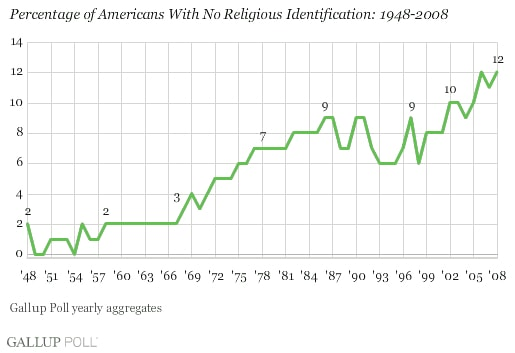
\includegraphics{./NonesRise.jpg}
\caption{Graph showing the rise of Americans with no religious
identification, from Gallup\autocite{GallupThisEasterSmaller}}
\end{figure}

To those believers, their religion does not just affect their actions
within a church or a mosque, but their religious beliefs make up a large
part of their world view. Religion shapes thoughts. Therefore, it makes
sense that understanding the religious beliefs of those around us is, in
general, a useful thing to do. However, at times, we might think that
discussing God or religion will be fruitless; that it will only end in
debate, shouting and, ultimately, an impasse. Just look to any online
comments section! (Figure 2)

\begin{figure}
\centering
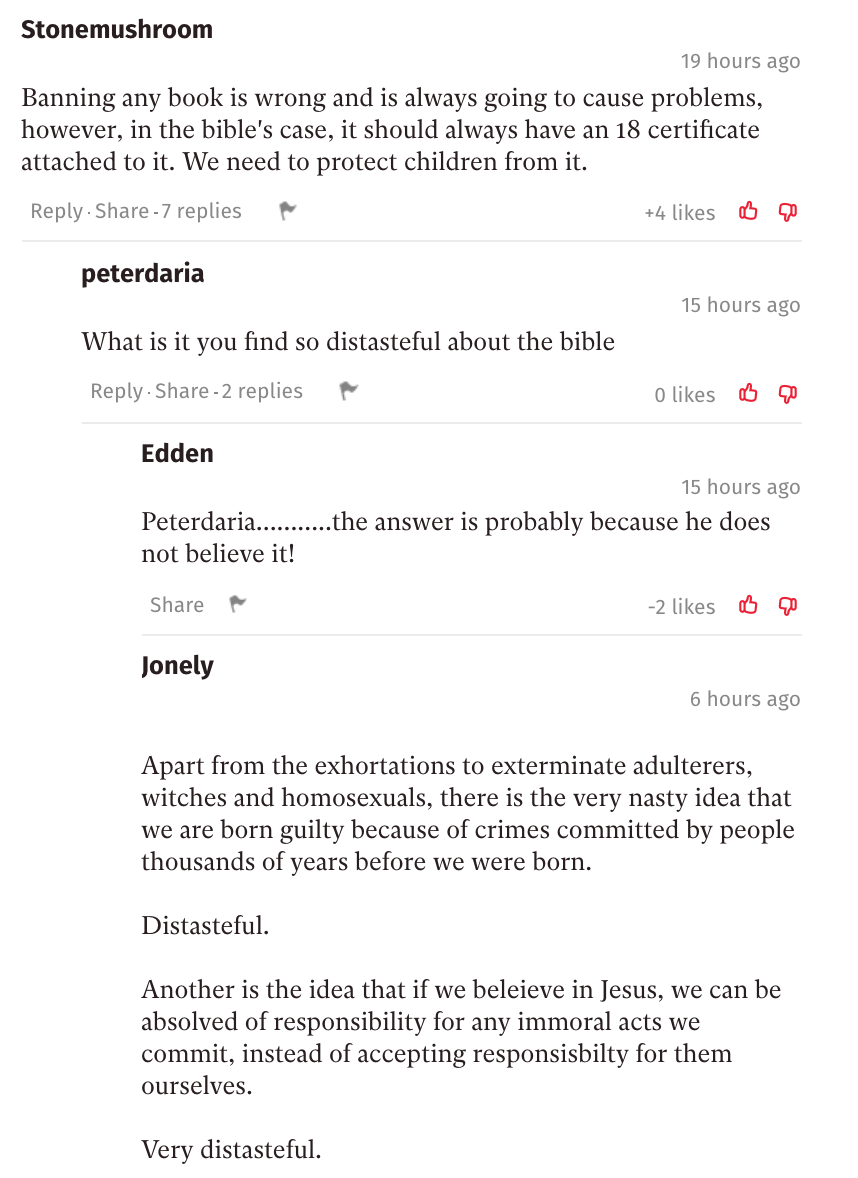
\includegraphics{./NewspaperComments.png}
\caption{A number of comments below an article on China's banning of the
Bible, found in 5 minutes from browsing the front page of \emph{The
Independant}.\autocite{OppenheimChinacrackssales2018}}
\end{figure}

But this is not a new issue. Herodotus, an Ancient Greek historian,
tells of a similar impasse when two groups discuss burial customs over
2000 years ago:

\begin{quote}
``When Darius was king, he summoned the Greeks who were with him and
asked them what price would persuade them to eat their fathers' dead
bodies. They answered that there was no price for which they would do
it. Then he summoned those Indians who are called Callatiae, who eat
their parents, and asked them (the Greeks being present and
understanding by interpretation what was said) what would make them
willing to burn their fathers at death. The Indians cried aloud, that he
should not speak of so horrid an
act''\autocite{HerodotusHistoryHerodotus1910}
\end{quote}

Karl Popper, in \emph{The Myth of the Framework}, rejects the notion
that this confrontation was fruitless. While he agrees that ``mutual
understanding was not
achieved''\autocite[pg 37]{PopperMythFrameworkdefence1997}, he points
out that even without conversation, this confrontation can begin to
breed tolerance and respect to those different from ourselves and, over
time, this can bear fruit; the fruit of
understanding"\autocite{PopperMythFrameworkdefence1997}.

While this example is extreme, it is a picture you might be scared of.
As you look at online comment sections, or at Richard Dawkins, or to
Israel \& Palestine, you might be put off by others' worldview. But
these extreme examples are the ones that stick out most in our mind
because we rarely actually see the beliefs and practices of those near
us. One's worldview, almost by definition, affects the way we see life,
and so affects what we do day-to-day. And yet, our clearest picture of
someone practising Islam (or, at least, their version of Islam) is found
in terrorist attacks, not in the practices of those close to us. The
comedian Lee Mack makes this point, when being interviewed on the BBC
Radio 4 show \emph{Desert Island Discs}:

\begin{quote}
``I think it's quite odd that people like myself, in their forties,
quite happy to dismiss the Bible, but I've never read it. I always think
that if an alien came down and you were the only person they met, and
they said, `What's life about? What's earth about? Tell us everything,'
and you said, `Well, there's a book here that purports to tell you
everything. Some people believe it to be true; some people {[}do{]} not
believe it {[}to be{]} true.' `Wow, what's it like?' and you go, `I
don't know, I've never read it.' It would be an odd thing wouldn't
it?''\autocite{BBCRadio4DesertIslandDiscs13}
\end{quote}

Mack points out the attitude of dismissing the Bible without examining
it is, at face value, an odd thing to do. While we may be scared off by
the actions of the religious, or we feel constrained by the taboo
religion holds, not bothering to ever look into it leaves us in the
dark; we end up distancing ourselves from the people around us.

As the Internet grew, people began to see it as a tool to bring people
together; as a tool to solve this exact issue. Way back in 1993,
internet theorist Michael Hauben wrote that ``The Net brings the
isolated individual into contact with people, opinions, and views from
the rest of the world''\autocite{HaubenNetNetizensImpact1993}. This, he
concludes, is an important aspect of the online world, since ``exposure
to many possible opinions gives the reader a chance to actually think
something over before making a decision as to a personal
opinion''\autocite{HaubenNetNetizensImpact1993}.

However, as the internet grew, each user's journey through the online
world was tailored just for them. Filter bubbles began to box us into
clusters, rather than exposing us to the world's opinions. From social
networks to search engines, the content we see was being categorized and
personalised. Eli Pariser, chief executive of Upworthy, in his book
\emph{The Filter Bubble}, wrote that as ``Google personalized for
everyone, the query `stem cells' might produce diametrically opposed
results for scientists who support stem cell research and activists who
oppose it''\autocite[pg 2]{PariserFilterBubblewhat2012}. When it comes
to religion, then, how can we push back against this
over-personalisation? How can we get back to an agora-like Internet,
where the world can meaningfully discuss issues of religion, philosophy
and worldview? In this piece, you will see a number of different ways of
approaching this issue; a number of differing voices, much like the
market place of ideas that the internet can offer. It is up to you to
decide which are meaningful, and which are not.

\begin{center}\rule{0.5\linewidth}{\linethickness}\end{center}

\textbf{The Christian}

Here, I want to address the Christian population. There is a tendency I
have noticed, both online and offline, for Christians to bubble off into
their own cliques and communities. In this piece, I seek to argue that
this tendency is not one that comes from the Bible and, in fact,
Christians should embrace an agora-like Internet as a chance to share
their faith.

To achieve this, it makes sense to use the text that unites the
Christian population - the gospels. These four books are four accounts
of the life of the central figure of Christianity, so turning to these
seems sensible. Here, for simplicity, we will use just two short
sections from the gospel of John. While there is little context in these
texts, both support one another in what they say. The first is chapter 3
verse 16, likely the most famous verse from John's gospel, often seen
around stadiums during American sports games. The verse itself is a
clear and concise description of Christ's role in the faith:

\begin{quote}
``For God so loved the world that he gave his one and only Son, that
whoever believes in him shall not perish but have eternal
life.''\autocite[pg 1035]{HolyBibleNew2007}
\end{quote}

\begin{figure}
\centering
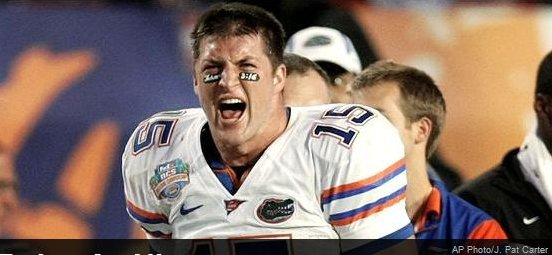
\includegraphics{./TimTebow.jpg}
\caption{American footballer Tim Tebow, with John 3:16 painted below his
eye during a playoff game}
\end{figure}

The second is chapter 30, verses 30 and 31. This comes near the end of
the gospel, and is an explanation by John as to why he curated the signs
(that is, miracles) of Jesus the way he did:

\begin{quote}
``Jesus performed many other signs in the presence of his disciples,
which are not recorded in this book. But these are written that you may
believe that Jesus is the Messiah, the Son of God, and that by believing
you may have life in his name.''\autocite[pg 1057]{HolyBibleNew2007}
\end{quote}

From these two verses we see three beliefs central to the Christian
faith:

\begin{enumerate}
\def\labelenumi{\arabic{enumi}.}
\tightlist
\item
  God has one son, Jesus, who he gave to the world.
\item
  This son, Jesus, is messianic. That is to say, he is some sort of
  saviour figure in Christianity.
\item
  If you believe in Jesus as the Messiah, and as God's Son, you can have
  eternal life in his name.
\end{enumerate}

The important belief to us here is the third. It is clear that belief in
Jesus is important to Christians; to believe in Jesus is to gain access
to an everlasting life after this one. Then, for the Christian, the role
of dialogue is to help others to know and understand Jesus. Some may
call this dialogue proselytizing. However, proselytizing brings up
images of megaphones on street corners; proselytizing is coercive and
pushy. Dialogue, on the other hand, is the Christian sharing their
faith, answering questions and so forth, in order to help people make up
their mind about Jesus properly. So, when Jesus says to ``love your
neighbor as yourself''\autocite[pg 956]{HolyBibleNew2007} in Matthew's
Gospel, I would call this form of dialogue more loving than the man
shouting on the street corner.

\begin{figure}
\centering
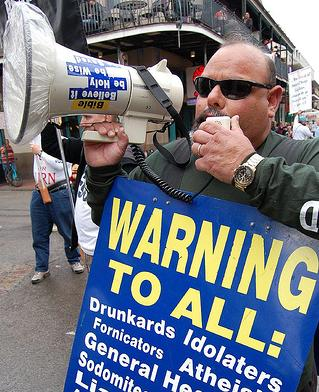
\includegraphics{./StreetPreaching.jpg}
\caption{A street preacher with a megaphone.}
\end{figure}

However, I would argue, to not share your faith as a Christian is also
an unloving act. In doing this, the Christian believes that they have
eternal life, yet they don't want anyone around them to have that life
also. Penn Jillette, Las Vegas magician and advocate for atheism, agrees
with this sentiment. In a video on the subject he said this:

\begin{quote}
``If you believe there is a heaven and hell, and people could be going
to hell or not getting eternal life or whatever, and you think it's not
really worth telling them this because it would make it socially
awkward\ldots{}How much do you have to hate somebody to not {[}tell
them{]}?'' \autocite{JilletteGiftBible2010}
\end{quote}

When we look online though, we see that it is easy for anyone, Christian
included, to stay in a bubble online. Eli Parisier, in \emph{The Filter
Bubble}, says that these exist because of the personalisation algorithms
found across the web. However, Parisier says, the bubble is ``a cozy
place, populated by our favorite people and things and
ideas''\autocite[pg 12]{PariserFilterBubblewhat2012}. Ultimately, like
anyone, Christians can be scared of what people will think of them, and
they don't like being challenged. In addition, with religion
specifically, this issue isn't solely who you engage with on Facebook;
almost all your media consumption can be within a Christian bubble. At a
conference, Mark Scott, the Former Managing Director of the Australian
Broadcasting Corporation, explained the issue as follows:

\begin{quote}
``The new media environment presents a great risk for Christians to
retreat. There will be in a media sense, a massive global market for
Christians to listen to Christian music, to read Christian books, to see
Christian films, to partake in Christian blogs, to comment on each
other's Christian Facebook pages and to live in that Christian
world.''\autocite{TaylorMarkScottChristians2014}
\end{quote}

For Christians then, there is tremendous comfort in staying within the
bubble, and there is enough media to allow you to stay there for as long
as you want to. Thus there seems to be a clash in the minds of
Christians, between (somewhat selfishly) staying within the bubble, and
(more selflessly) sharing your faith for the sake of those around you.

This clash can be seen in a 2017 study by Brubaker and
Haigh\autocite{BrubakerReligiousFacebookExperience2017}. In the study,
335 Christians participated in an online study about their engagement in
religious content and community online. With regards to how much
Christians see Facebook as a platform for dialogue, they found that
``those who use {[}Facebook{]} for religious purposes recognize the
potential for visibility and therefore reach out to people with diverse
beliefs and varying commitments to those
beliefs''\autocite[pg 8]{BrubakerReligiousFacebookExperience2017}.
However a second, more interesting insight is that ``people who were
more religious were also more likely to minister to others
online''\autocite[pg 9]{BrubakerReligiousFacebookExperience2017}. This
seems to back our hypothesis above; those who are more religious are
more certain of an everlasting life after this one, so will think it
more crucial to try to tell people about Jesus, and that new life. In
contrast, those who are less sure themselves, are more likely attracted
to the comfort the bubble provides, rather than sticking their neck out
for the sake of those around them.

So, from this, we have seen that the Bible backs up the case for
dialogue (rather than proselytizing), and yet Christians are conflicted.
On the one hand, they want to start a dialogue out of a sense of love
for those around them. Yet, there is comfort in staying still, and
dangers (either percieved or real) of sharing their faith online. It is
my opinion, then, that we need to teach Christians what the Bible says
about dialogue. As online personalisation seems to be only getting
stronger, Christians will have a tendency to clump together, unless we
can help them understand why that tendency is an unbiblical one.

\begin{center}\rule{0.5\linewidth}{\linethickness}\end{center}

\textbf{The Network Theorist}

'Birds of a feather flock together" as the saying goes. This is
homophily; the tendency of individuals to associate with those similar
to them. While homophily is hardly a new concept, the dawn of social
networks provided an extensive dataset to study the area. In 2008,
Thelwall looked at a sample of 2,567 members of Myspace to see patterns
of behaviour\textsuperscript{21}. While he found no evidence of
homophily within genders, he found significant evidence of homophily in
many other areas, including within religions\textsuperscript{22}.
However, social networks do more than just provide data; they change the
very nature of the connection between members within the network. In
this piece, I seek to show that individual tendency, coupled with the
structure of social networks (looking at Facebook specifically), only
seeks to clump people together. In addition, I propose two possible
areas that could successfully push back against this model.

In \emph{The Filter Bubble}, Parisier says that online filter bubbles
``tend to dramatically amplify confirmation bias''\textsuperscript{23}.
Since we naturally become frustrated by information that challenges our
assumptions, we tend to instead drift towards information that we agree
with. Thus, we have a tendency toward those who hold a similar viewpoint
to us; those of the same religion, or even of the same denomination
within that religion. And, since online filter bubbles personalise, they
amplify things we have a tendency towards, so amplifying this
confirmation bias\textsuperscript{24}.

But how does this compare to the offline world of homophily? Take the
example of stratified housing communities, where the rich and the poor
live in different districts. Each district is like it's own filter
bubble, amplifying confirmation bias within it. However, the difference
lies in the fact that each member is not confined to their own district.
Naturally, people live in different contexts, and move between these
contexts daily. While these contexts may be related (those who are rich
may have different hobbies to those who are poor), each context is
skewed in different ways (as can be seen in Figure 5). So, while your
affinity toward certain people still exists (as seen by the thickness of
the lines in the figure), you end up interacting with people from
different religious beliefs.

\begin{figure}
\centering
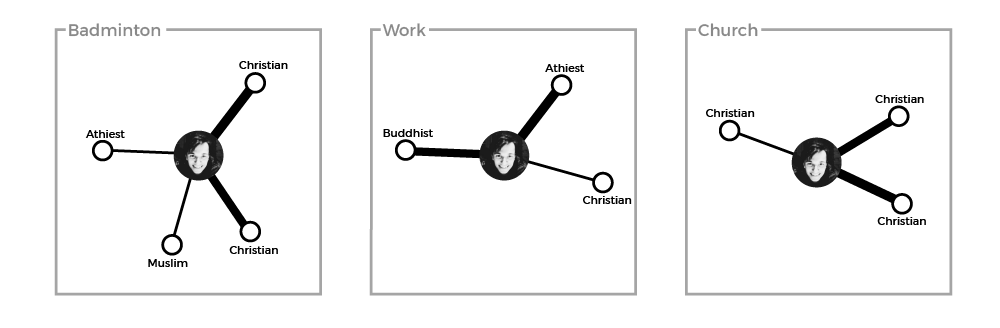
\includegraphics{./NetworkDiagram1_1.png}
\caption{Offline contexts of a Christian, with affinity toward a person
indicated by line thickness}
\end{figure}

In the offline world, however, you hold one identity - one profile.
Facebook founder, Mark Zuckerberg told journalist David Kirkpatrick for
his book \emph{The Facebook Effect:}

\begin{quote}
``The days of you having a different image for your work friends or
coworkers and for the other people you know are probably coming to an
end pretty quickly.''\textsuperscript{25}
\end{quote}

So it makes sense that, on Facebook, there is one context where you have
no direct control. And, when all the contexts are aggregated (see Figure
6), online filter bubbles amplify those you have an affinity for. We see
then that, online, your feed becomes skewed towards views similar to you
in a different way to the offline world.

\begin{figure}
\centering
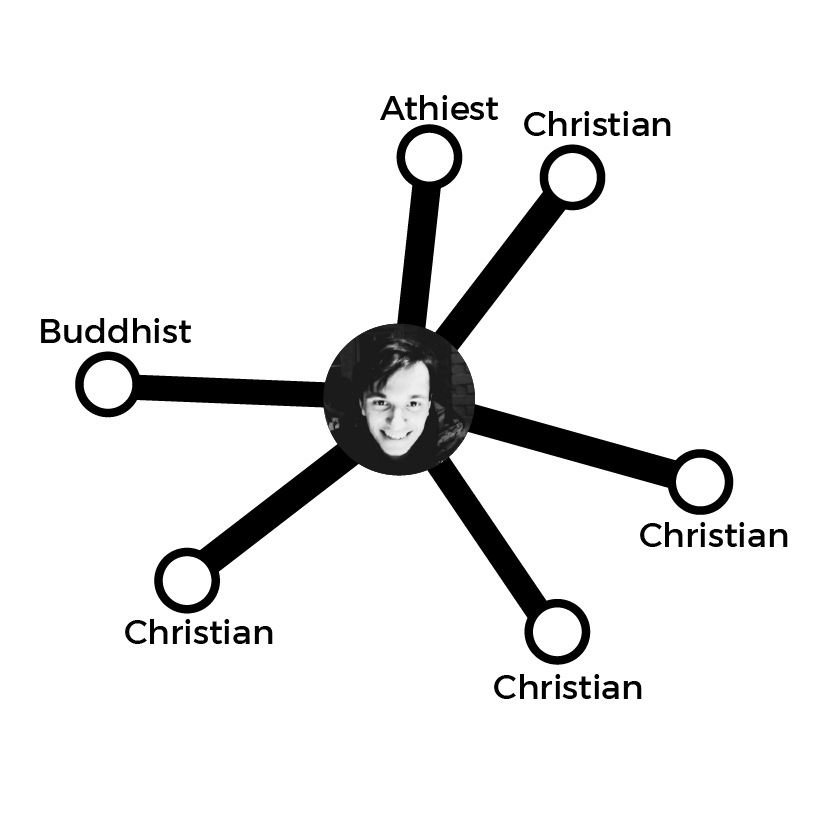
\includegraphics{./NetworkDiagram1_2.png}
\caption{The aggregation of offline contexts onto a single online
profile. Now, affinity towards other Christians shows up much more
starkly, since these are the only people you see in your feed.}
\end{figure}

However, within this network, it might seem surprising that the number
of hops between you and every other member is actually very small. In a
2011 analysis of the Facebook network, they found that 99.6\% of users
are connected in 6 links or less, with the average distance being 4.7
links\textsuperscript{26}, as seen in the graph in Figure 7. At the same
time, though, they found that the amount of clustering in Facebook is
very high. In the literature, clustering is measured as a coefficient
between 0 and 1. A coefficient of 1 indicates that all of your friends
are also friends with each other. In the 2011 analysis, they concluded
that ``for users with 100 friends, the average local clustering
coefficient is 0.14, indicating that for a median user, 14\% of all
their friend pairs are themselves friends''\textsuperscript{28}. This
coefficient as found to be ``five times greater than the clustering
coefficient found in a 2008 study analyzing the graph of MSN messenger
correspondences, for the same neighborhood size'' \textsuperscript{29}.

\begin{figure}
\centering
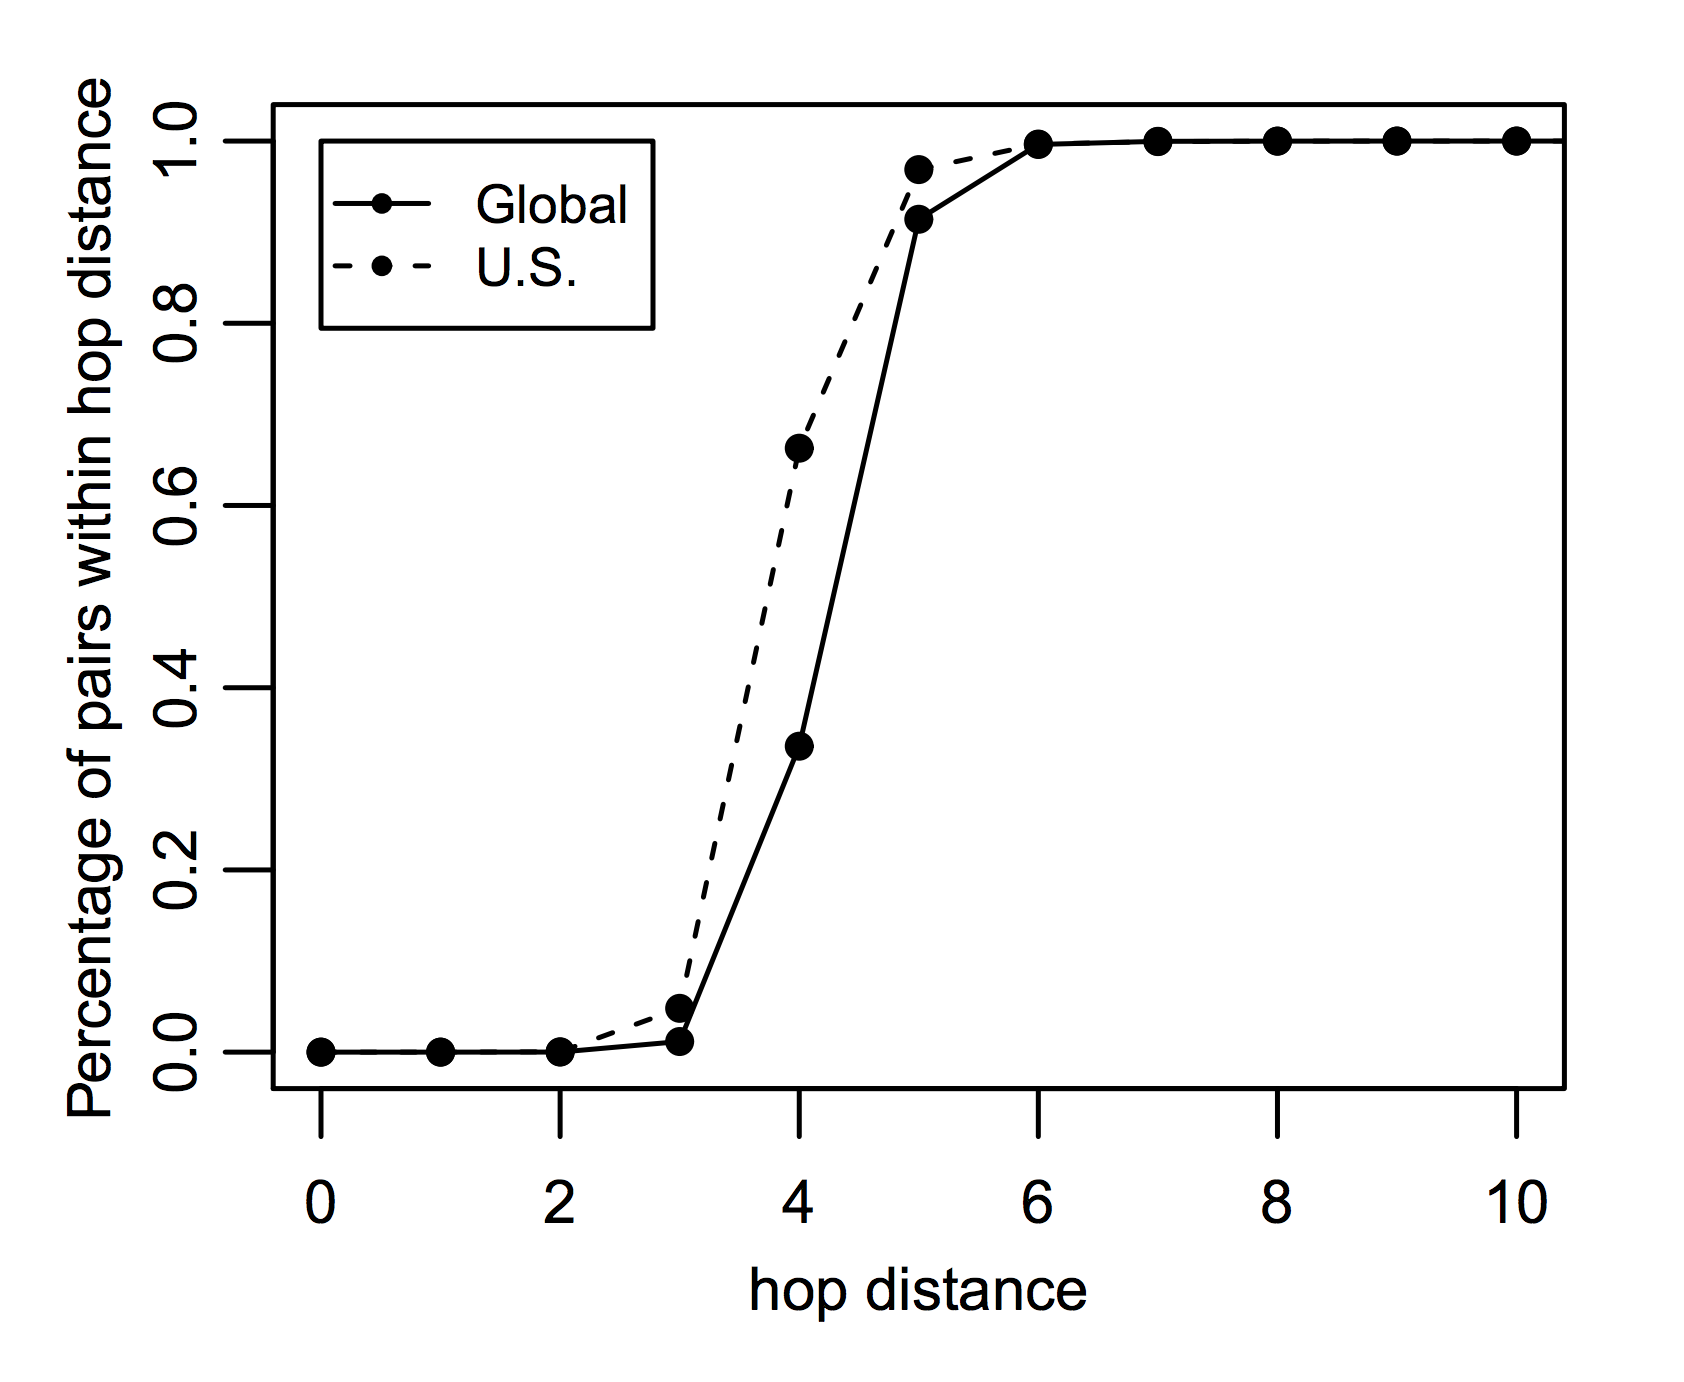
\includegraphics{FBLinks.png}
\caption{Graph showing the percentage of user pairs that are within
\emph{h} hops of each other, from Ugander et al.\textsuperscript{27}}
\end{figure}

This apparent contradiction is explained by a seminal paper by Strogatz
and Watts\textsuperscript{30}. Here they called these networks, with a
high amount of clustering and a small average path length,
`small-worlds' networks\textsuperscript{31}. These networks are ``caused
by the introduction of a few long-range edges''\textsuperscript{32};
individuals who have a supremely large number of links within the
network. These individuals, who we will call `hubs', become the `glue'
between disparate clusters. So, then, one approach to stop
over-personalisation might be to harness the power of these hubs. While
clustering is very high within the network, the 2011 study found an
interesting insight when studying friends-of-friends. While you would
expect the average user with 100 friends to have ``100∗99 = 9,900
non-unique friends-of-friends''\textsuperscript{33}, they found that
they have far more than that; ``27,500 unique friends-of-friends and
40,300 non-unique friends-of-friends''\textsuperscript{34}. This is
likely due to the these hubs in the network. While most of your friends
will have a similar number of friends as you, a small number are
incredibly well-connected, which explains why you have so many more
friends-of-friends than expected.

However, rather than playing this up, social networks tend to play this
down. Parisier, in \emph{The Filter Bubble}, looked at Twitter. He found
that:

\begin{quote}
``Twitter users see most of the tweets of the folks they follow, but if
my friend is having an exchange with someone I don't follow, it doesn't
show up. The intent is entirely innocuous: Twitter is trying not to
inundate me with conversations I'm not interested in. But the result is
that conversations between my friends (who will tend to be like me) are
overrepresented, while conversations that could introduce me to new
ideas are obscured.''\textsuperscript{35}
\end{quote}

So, then, one method would be to push against this shift within our
social networks, by allowing users to see interactions between their
friends and people they don't know, to give a springboard for
conversation with those outside your immediate cluster.

Coming back to contexts, a second method could be to split the internet
back into different contexts, while Facebook (among others) tend to
group them together. An example is the forum site Reddit, where there
are a number of smaller forums (called subreddits). The front page of
the subreddits you join are aggregated, to form your feed. The
difference with this compared to Facebook, for example, is that your
feed is not altered based on which subreddits you look at regularly, so
your experience is much more broad.

The issue here is one of framing. Imagine a user joins the subreddit for
badminton players, and the subreddit for Christians. This may not seem
like a problem, because these two communities are disparate; badminton
players are religiously diverse, and Christians play a lot of different
sports. However, subreddits are framed in a certain way; the badminton
subreddit is devoted to badminton, and the Christianity subreddit is
devoted to Christianity. Almost by definition, discussion on the
badminton subreddit is devoted to badminton, while discussion on
Facebook with your badminton friends, on the other hand, can be diverse.
This is likely because you are more comfortable around those friends you
play badminton with in the offline world; you know them personally, and
so want to find out about their life as a whole. However, the same
cannot be said about faceless users of a badminton forum.

The conclusion then might be to create new contexts online. A good
example is the DebateReligion subreddit\textsuperscript{36}, where users
(you guessed it) discuss and debate religious topics, or
ChangeMyView\textsuperscript{37}, a more general subreddit for
discussing perspectives on different opinions. These subreddits are
designed as agora-like forums, to discuss and debate ideas. It is a rosy
picture, but the issue here is one of size. While ChangeMyView and
DebateReligion have roughly 600,000 combined subscribers, there are over
2 billion active Facebook users\textsuperscript{38}. The user base of
these subreddits make up just 0.03\% of the user base of Facebook.
However, the model of specific communities of strangers dedicated to
understanding one another is a useful one.

Parisier proposes a happy medium between the ghetto-like model of
Facebook and the agora-like model of Reddit. Comparing the internet to a
city, he says that ``we need our online urban planners to strike a
balance between relevance and serendipity, between the comfort of seeing
friends and the exhilaration of meeting strangers, between cozy niches
and wide open spaces''\textsuperscript{39}. The network structure of
Facebook is flawed; it clumps all those you know together, and then
amplifies the connection you feel towards those who hold the same
beliefs you do. It creates, as Parisier says, a ``city of
ghettos''\textsuperscript{40}. However, either by context splitting, or
by harnessing the power of hubs in the network, we can strive to create
a better city, where internet citizens are given a space to think and
discuss the most important questions of human existence.

\begin{center}\rule{0.5\linewidth}{\linethickness}\end{center}

\begin{enumerate}
\def\labelenumi{\arabic{enumi}.}
\setcounter{enumi}{20}
\tightlist
\item
  Thelwall, Mike. 2009. ``Homophily in MySpace.'' \emph{Journal of the
  American Society for Information Science and Technology} 60 (2):
  219--31. \url{https://doi.org/10.1002/asi.20978}, pg 219.
\item
  ibid., pg 229
\item
  Pariser, Eli. 2012. \emph{The Filter Bubble: What the Internet Is
  Hiding from You}. London: Penguin Books, pg 88
\item
  ibid.
\item
  Kirkpatrick, David. 2011. \emph{The Facebook Effect: The Inside Story
  of the Company That Is Connecting the World}. 1st Simon \& Schuster
  trade pbk. ed. New York: Simon \& Schuster Paperbacks, 199
\item
  Ugander, Johan, Brian Karrer, Lars Backstrom, and Cameron Marlow.
  2011. ``The Anatomy of the Facebook Social Graph.''
  \emph{ArXiv:1111.4503 {[}Cs.SI{]}}, November.
  \url{http://arxiv.org/abs/1111.4503}, pg4-5.
\item
  ibid., pg 4, figure 2.
\item
  ibid., pg 6
\item
  ibid.
\item
  Watts, Duncan J., and Steven H. Strogatz. 1998. ``Collective Dynamics
  of `Small-World' Networks.'' \emph{Nature} 393 (6684): 440--42.
  \url{https://doi.org/10.1038/30918}.
\item
  ibid., pg 440
\item
  ibid., pg 440
\item
  Ugander, Johan, Brian Karrer, Lars Backstrom, and Cameron Marlow.
  2011. ``The Anatomy of the Facebook Social Graph.''
  \emph{ArXiv:1111.4503 {[}Cs.SI{]}}, November.
  \url{http://arxiv.org/abs/1111.4503}, pg8.
\item
  ibid.
\item
  Pariser, Eli. 2012. \emph{The Filter Bubble: What the Internet Is
  Hiding from You}. London: Penguin Books, pg 150
\item
  ``DebateReligion.'' n.d. Reddit. Accessed April 8, 2018.
  \url{https://www.reddit.com/r/DebateReligion/}.
\item
  ``Change My View (CMV).'' n.d. Reddit. Accessed April 8, 2018.
  \url{https://www.reddit.com/r/changemyview/}.
\item
  Statista. n.d. ``Facebook Users Worldwide: 2017.'' Statista: The
  Statistics Portal. Accessed April 8, 2018.
  \url{https://www.statista.com/statistics/264810/number-of-monthly-active-facebook-users-worldwide/}.
\item
  Pariser, Eli. 2012. \emph{The Filter Bubble: What the Internet Is
  Hiding from You}. London: Penguin Books, pg 222
\item
  ibid.
\end{enumerate}

\begin{center}\rule{0.5\linewidth}{\linethickness}\end{center}

\textbf{What stops us using Bohm Dialogue in online religious dialogue?}

When discussing how to use theories of dialogue to facilitate meaningful
online covnversation, we must first examine the characteristics of a
theory of dialogue. For this, we will use the theory put forth by David
Bohm, in his book \emph{On Dialogue} (INL\_Bohmbook). The initial
distinction made by Bohm is between discussion and dialogue. Bohm points
out that the word discussion has ``has the same root as `percussion' and
`concussion'.'' (INL\_Bohmbook\_7), and so emphasises breaking things up
and analyzing them, in order to come to one consensus. This, he says,
leads to ``a ping-pong game'' (INL\_Bohmbook\_7), where individuals are
aiming to score points for your side. Dialogue, on the other hand, comes
from two roots - ``\,`dia' which means `through' and `logos' which means
`the word', or more particularly, `the meaning of the
word.'\,''(INL\_Bohmsite). This conjures the image of a river of
meaning, flowing through and around individuals engaged in dialogue.
Bohm proposes that this flow of shared meaning does two things. Firstly,
is creates a new understanding between participants, where before (with
discussion) there was a divide. Secondly, it focuses on creating
something new - a new flow of shared meaning.

To create this kind of dialogue, assumptions must be addressed. When
individuals come together, there will be a variety of held assumptions
and opinions underlying the conversation. When a particular assumption
from one member comes up, another member may be angry, for example with
the Greeks and the Callatiae seen in the Introduction. Bohm calls
members in dialogue to `suspend' an angry reaction (unkind words, for
example). This `suspension', Bohm says

\begin{quote}
``involves exposing your reactions, impulses, feelings and opinions in
such a way that they can be seen and felt within your own psyche and
also be reflected back by others in the group'' (INL\_Bohmsite)
\end{quote}

On the one hand, this allows you to feel like you have sated the anger
in some way and, on the other, it allows the group to give serious
examination to why individual thoughts and assumptions give rise to
strong emotions and feelings (INL\_Bohmsite). While Bohm says that
religious dialogue is often the most difficult, this notion of
suspension helps tremendously. In discussion or debate, individuals are
trying to convince the group of some kind of truth position (a religious
one, or otherwise). However, Bohm dialogue recognizes there will be
clashes and anger over certain issues and certain assertations. So,
through suspension, it seeks to help members explore where this anger
comes from.

This new model of dialogue, where focus is on shared meaning and
suspending reactions to others' opinions, is set out to work in the
general case. However, in our context, there is a barrier we need to
examine. The online world is markedly different to the offline world
Bohm was writing in, and these changes pose problems to dialogue, as
well as creating new opportunites for it. We will examine the
application of Bohm dialogue in the online world.

One major area is anonymity and masking. Some platforms are wholly
anonymous. In a forum or in a game, for example, users create a new
avatar for themselves that can be similar or different to their offline
self. In some ways, this anonymity allows for more open dialogue. In a
2001 study (INL\_JOINSON), students were asked to talk about personal
questions in pairs; some pairs spoke in person, while others spoke
anonymously though an instant messaging program. After this study, it
was concluded that the online students ``disclosed signifcantly more
about themselves'' (INL\_JOINSON\_181) that those who were face-to-face.
In many ways this makes sense. There are a number of social behaviours
dictating behaviour in offline conversation, while those pressures are
almost abstracted away when conversation just becomes text on a screen.
However this can have a negative side also. When, for example, Bohm asks
people to suspend their angry reaction to someone's opinion, there is a
social pressure to do that, especially since rude words and shouting is
mostly frowned up in conversations. However, those pressures don't have
the same weight in the offline world, due to the abstraction of the
interface. This is likely why we often see arguments below news stories
and YouTube videos.

In many ways, the situation is similar in non-anonymous platforms (such
as messaging friends, or using social media). While we may know the
person, there is still some sort of abstraction. Seeing someone we know
in person makes us tighten up to social pressures, while interacting
with them on the internet makes us freer on the whole. Another important
thing to examine is why people use social media. An example is a 2011
study, which examined why people use Facebook (INL\_Nadkarni). They
found that Facebook use is motivated both by the need to belong, and by
the need for self-presentation. The first of these gives rise to
relationship and community bonding. The second gives rise to holiday
photos and bragging. The combination of these, however, is not dialogue.
Instead, individuals become part of a community, and then are afraid
discuss anything challenging that community. So then, while the nature
of the internet does in part allow for freer conversation, relational
social media sites can give rise to tight communities, not dialogue.

Another issue is how information is displayed. In Bohm Dialogue, the
``basic notion\ldots{}would be for people to sit in a circle {[}since{]}
such a geometric arrangement doesn't favor anybody''(INL\_Bohmbook\_17).
In social networks this is often not the case. The `sitting' in the
online space is akin to what we see when we login to the platform. Most
platforms show us, at least automatically, content based on one of two
factors. The first is what most interests us -- found on YouTube, and
the majority of the screen on Twitter and Facebook. This is usually
based on machine learning algorithms which learn which content we are
most likely to click, share or like. The second is what is most popular
among the whole of the network (in other words, what is trending) --
found on Reddit, as well as a smaller section of the screen on Twitter
and Facebook. But this arrangement does favour certaing people. In the
first, it favour people with views that are more popular to the most
number of people. In the second, it favours those that are popular among
the whole network. This leads to, on the whole, populists being favoured
in internet discussions. I would suggest that a more democratic, more
`circle-like' configuration may be to prioritise by the newest content.
The issue here is that this approach will likely cause users to spend
less time on the site when compared with the other approaches, since the
latter is designed, through software, to keep us on the site longer.
This is evidenced by the fact that many social networks are beginning to
sort their feeds by this latter approach. Twitter, for example, changed
the makeup of its timeline in February 2016, with it now ``designed to
{[}show{]} the best tweets that users may have missed based on what
Twitter thinks you care about'' (INL), rather than showing the most
recent tweets.

\end{document}
